\chapter{Event reconstruction}

\intro{The reconstruction of basic analysis objects within an event is described. A key ingredient in the \gls{cms} reconstruction is the particle flow algorithm which defines particle candidates by combining various subdetector information. The focus is set on the reconstruction and performance of muons, electrons, jets, and the missing transverse energy in 8 and 13~TeV pp~collision data which are the input objects in this thesis to study single top quark production.}

The event reconstruction attempts to reconstruct and identify basic analysis objects from the raw detector data. In \gls{cms}, basic objects are particle tracks and vertices as well as charged lepton, photon, and jet candidates. During the reconstruction additional information such as the missing transverse energy, $\met$, and the likelihood of jets to originate from the hadronization of b~quarks~(``b-tagging'') is determined. Since $\tau$ leptons and photons are not relevant for the study of $t$-channel single top quark production a description of their reconstruction and performance is omitted here yet details can be found in Refs.~\cite{Khachatryan:2015iwa,Khachatryan:2015dfa}.


%##############################################
\section{Track reconstruction}
%##############################################

The track reconstruction is split in two steps. First, in the local reconstruction, hits from charge distributions on the pixel and strip modules of the tracker are formed. Then, in the global reconstruction, trajectory candidates are seeded and build from compatible hits. A curved track is fitted to the found hits while accounting for the magnetic field to estimates parameters like the particle's momentum and charge. The individual steps are described briefly in the following. More details can be found in Ref.~\cite{Chatrchyan:2014fea}.

Different algorithms are used to determine the local position of two-dimensional (one-dimensional) hits from the distributions of charge deposits on the pixel (strip) modules respectively. For pixel hits, a fast estimation of the hit position is performed first which is utilized in the trajectory seeding and building stage only. Here, the 2D charge distribution is projected onto each axis and the position is estimated from the deposited charges at the edge of a charge cluster while accounting for the Lorentz-drift in the modules. During the track-fit, the optimal pixel hit position is estimated by comparing the charge distribution against simulated templates for various incident angles~\cite{Swartz:2007zz}. In the barrel layers, the pixel hit resolution is measured as $9.4~\upmu\mathrm{m}$ in $\mathrm{r}\phi$ and ranges between $21\range45~\upmu\mathrm{m}$ along the z-axis depending on the incident angle~\cite{Chatrchyan:2014fea}. 

For the strips, charge clusters are formed if the channel readout of adjacent strips is sufficiently above their individual noise levels. The hit position is then calculated as a charge-weighted average over a cluster and corrected for the Lorentz drift and potential inefficiencies occurring at the module edges. The hit resolution depends largely on the cluster size and pitch of the modules. It ranges roughly between $10\range30~\upmu\mathrm{m}$ and $10\range50~\upmu\mathrm{m}$ for the \gls{tib} and \gls{tob} modules respectively~\cite{Chatrchyan:2014fea}.

Track reconstruction is performed in multiple passes, called iterations, over the reconstructed hits to reduce the combinatorial complexity. Each iteration consists of the same algorithmic steps~(seeding, trajectory finding, track fitting, and selection) but is configured differently. The first iterations attempt to reconstruct only simple tracks which originate close to the interaction region and have a sufficiently large transverse momentum. The hits belonging to successfully reconstructed tracks are masked in subsequent iterations which reduces the combinatorics. Later iterations focus then on displaced or low momentum tracks which may not originate from the interaction region using the remaining hits. Figure~\ref{fig:reconstruction-trackingiter} shows the efficiency and acceptance for successfully reconstructing a track\footnote{Tracks are reconstructed ``successfully'' if at least 75\% of their hits can be associated to a simulated particle.} in simulation, broken down per iteration, as a function of its transverse momentum and displacement.

\myfigure{\label{fig:reconstruction-trackingiter}Efficiency and acceptance of successfully reconstructing a track in simulation per tracking iteration as a function of (a)~the transverse momentum and (b)~the transverse displacement. The figures are taken from the public tracking result web page of CMS~\cite{trackingpublic}.}{
\subfloat[]{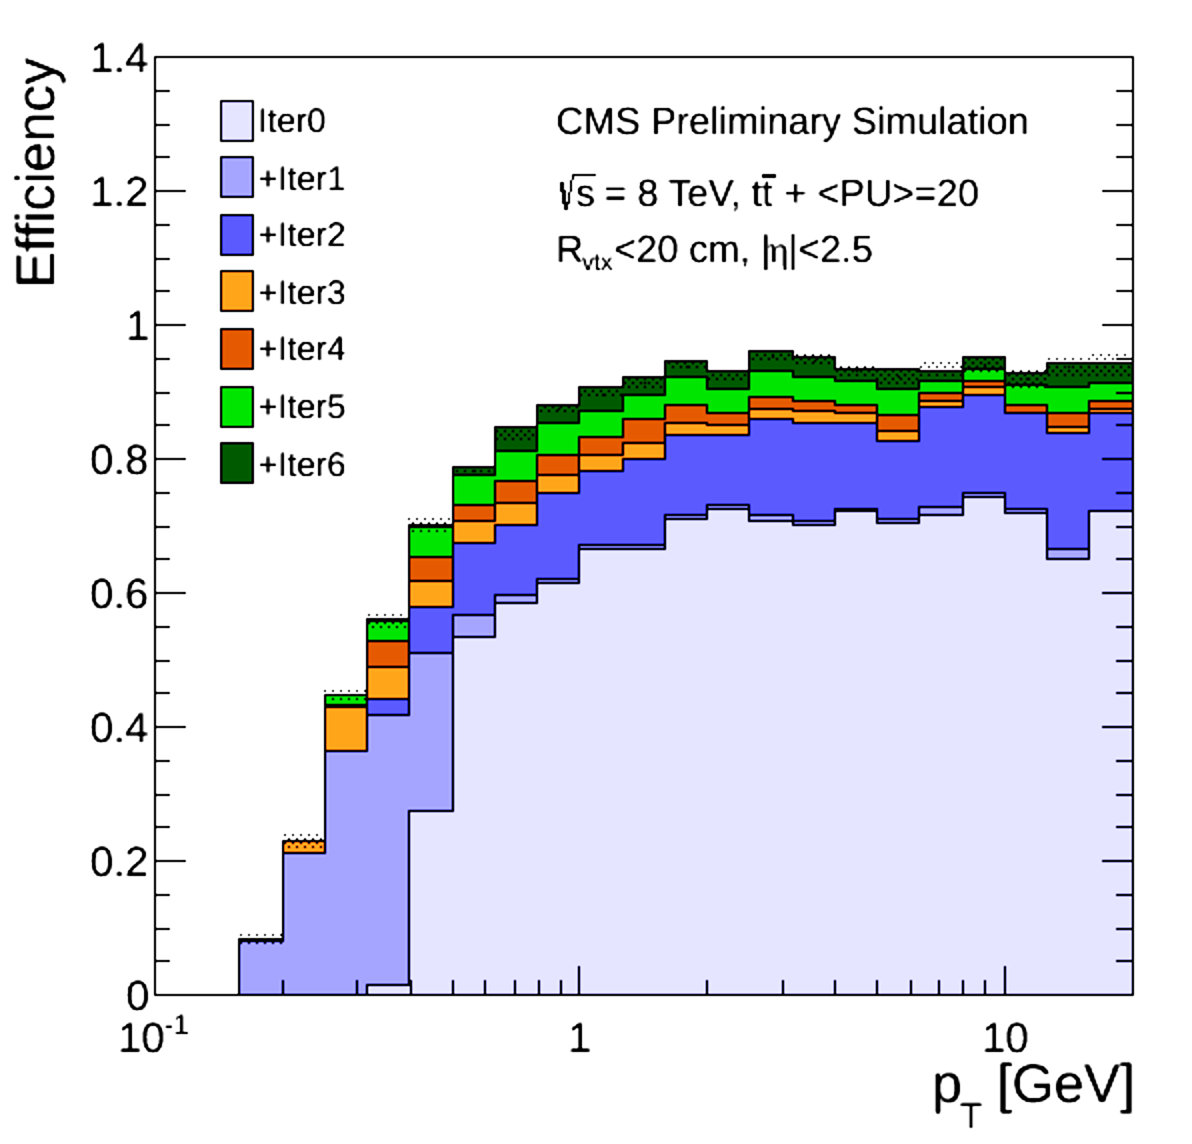
\includegraphics[width=0.48\textwidth]{figures/reconstruction/tracking_vs_pt.jpg}}\hspace{0.03\textwidth}
\subfloat[]{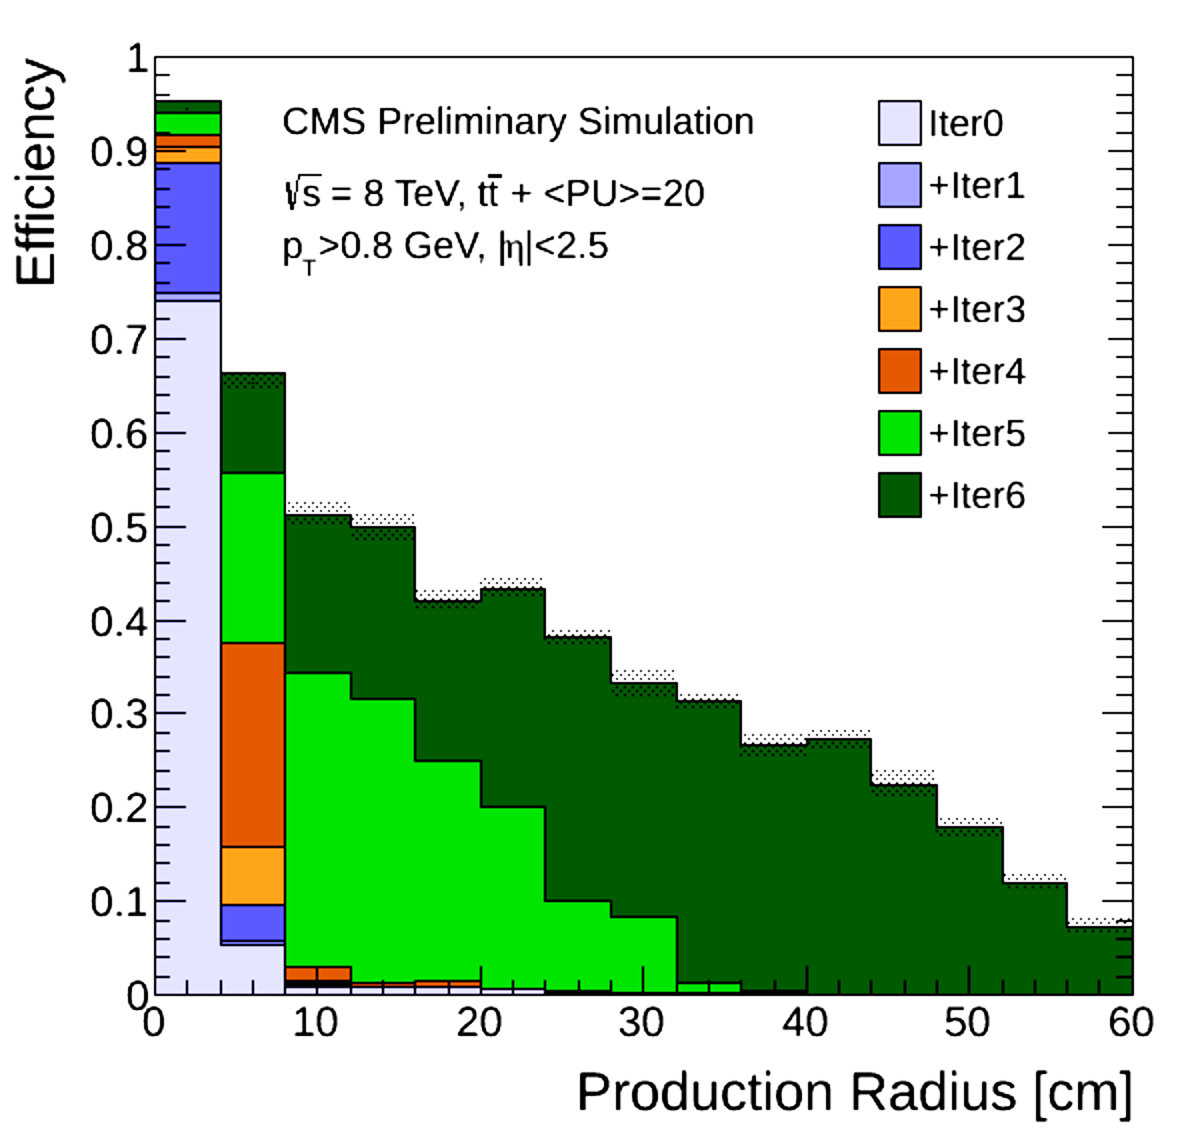
\includegraphics[width=0.48\textwidth]{figures/reconstruction/tracking_vs_vertpos.jpg}}
}

A trajectory seed is formed from a hit doublet or triplet where only certain combinations of tracker layers depending on the iteration are allowed for the hits. First iterations utilize mostly 3D hits on the pixel layers for seeding since their low channel occupancy results in less ambiguity and a higher efficiency for close-by tracks. Late iterations use hits on the strips instead where the spatial track density is low. Here 3D matched hits are utilized mostly which stem from double-sided strip modules but also mono layers are allowed. A seed candidate has to fulfill certain quality criteria depending on the iteration such as a minimal transverse momentum and compatibility with either the beam spot or a preliminary reconstructed vertex.

Each seed contains enough information to commence a first estimate of the track parameters. An algorithm called \gls{ctf} extrapolates the trajectory to find additional hits on subsequent layers which are compatible with the track hypothesis. It is based on the \gls{kf} technique which describes how to update the track parameters and their uncertainties iteratively after adding a hit. If multiple hits are found to be compatible with the track, new trajectories are generated for each of them. In the case no compatible hit is found on a layer a ghost hit is created instead.

The hits per trajectory are then passed to a \gls{kf}-based track fit to estimate the track parameters without utilizing the initial estimate from the seed. In addition, the fit accounts for material effects and the inhomogeneous magnetic field.  The fitted tracks have to pass a quality selection to reduce the amount of fake tracks before they can be considered in physics analyses. The criteria reflect the seed requirements and depend additionally on e.g. the total number of (3D) hits, the $\chi^2/\mathrm{\gls{ndof}}$ of the fit, the amount of ghost hits, the amount of shared hits with other tracks, amongst others.

The tracking efficiency for isolated muons with $1<\pt<100~\GeV$ is found to be above $99\%$ over the full tracker acceptance since their trajectories is only disturbed by energy loss and Coulomb scattering. The trajectory of charged hadrons, like pions, is additionally affected by nuclear interactions especially at low momenta ($\pt<700~\MeV$) which yields efficiencies between $80\range95\%$~\cite{Chatrchyan:2014fea}. For electrons a special tracking is performed in addition to account for their energy loss via bremsstrahlung as described in Sec.~\ref{sec:reconstruction-electrons}. In parts of the 2016 collision data, the overall tracking efficiency decreased by about 10\% at high instantaneous luminosities~(\todo{how high}) due to a charge saturation effect on the readout chips leading to missing hits~\cite{CMS-DP-2016-043} which however was recovered by changing the drain speed.


%##############################################
\section{Vertex and beam spot reconstruction}
%##############################################


The vertex reconstruction tries to locate points of pp interactions by finding tracks that originate from a common point within uncertainties. For this track are selected that originate closely from the beam spot and have a high reconstruction efficiency. Selected tracks are clustered using deterministic annealing~\cite{726788}. Here the association of a track to a vertex candidate is floating and modeled by a probability. A model similar to statistical mechanics is created where each track reflects a microstate. The free energy of the system is given by

\begin{align}
F&=-T\sum_{i}^\mathrm{tracks}p_{i}\log\left[\sum_{k}^\mathrm{vertices}\rho_{k}\,\mathrm{exp}\big(-\Delta_{ik}(T)\big)\right]\\
p_{ik}&=\frac{\rho_{k}\,\mathrm{exp}\big(-\Delta_{ik}(T)\big)}{\sum_{k\prime}\rho_{k\prime}\,\mathrm{exp}\big(-\Delta_{ik\prime}(T)\big)},\qquad\Delta_{ik}(T)=\frac{1}{T}\frac{(z_{i}^\mathrm{track}-z_{k}^\mathrm{vertex})^2}{\sigma_{z\,i}^{2}}
\end{align}

where $\sigma_{z}$ denotes the track resolution and $p_{ik}$ the track-vertex assignment probabilities. The initial compatibility of a track with the beam spot is encoded in the constant weights $p_{i}$. The temperature is decrease iteratively until a certain temperature is reached. New vertices are added if a minimum of $F$ is reached thus turning it into a saddle point instead. The final vertex positions are estimated through a fit using the clustered tracks.




%##############################################
\section{Particle flow}
%##############################################

%##############################################
\section{Muons}
%##############################################

id, trigger

%##############################################
\section{Electrons}
%##############################################
\label{sec:reconstruction-electrons}

gsf, id

%##############################################
\section{Jets}
%##############################################

CHS, JEC, JER

%##############################################
\section{b-tagging}
%##############################################

csv, SF, rizzi recipe

%##############################################
\section{Missing transverse energy}
%##############################################

T0, T1 corrections

%##############################################
\section{Luminosity and pileup}
%##############################################

pileup, rho
